\documentclass{article}
\usepackage{arxiv}

\usepackage[T2A]{fontenc}
% \usepackage[T1]{fontenc}
\usepackage[utf8]{inputenc}
\usepackage[english, russian]{babel}

\usepackage{url}
\usepackage{booktabs}
\usepackage{amsfonts}
\usepackage{nicefrac}
\usepackage{microtype}
\usepackage{lipsum}
\usepackage{graphicx}
\usepackage{natbib}
\usepackage{doi}

\usepackage{wrapfig}
\usepackage{titlesec}
\usepackage[inkscapeformat=png]{svg}
\usepackage{adjustbox}
\usepackage{caption}
\usepackage{subcaption}
\usepackage{graphicx}
\usepackage{multirow}

\usepackage{algorithm}
\usepackage{algpseudocode}
\usepackage{amsfonts}
\usepackage{amssymb, amsmath, mathrsfs, amsthm}
\usepackage{bbm}
\usepackage{bm}
\usepackage{color}
\usepackage{csvsimple}
\usepackage{fancyvrb}
% \usepackage[hidelinks]{hyperref}
\usepackage{indentfirst}
\usepackage{listings}
\usepackage{mathtools}
\usepackage{pgfplots}

\usepackage{algorithm}
\usepackage{algcompatible}
\usepackage[nottoc]{tocbibind}

\graphicspath{{../figures/}}


\title{Разработка эффективной реализации методов, основанных на поиске оптимального баланса между дивергенцией и точностью аппроксимации}

\author{ Аристархов Данила Дмитриевич \\
	ВМК МГУ \\
	\texttt{aristarkhov.danila@yandex.ru} \\
	%% examples of more authors
	\And
	Сенько Олег Валентинович \\
	ВМК МГУ \\
	\texttt{senkoov@mail.ru} \\
}
\date{}

\renewcommand{\shorttitle}{\textit{arXiv} Template}

%%% Add PDF metadata to help others organize their library
%%% Once the PDF is generated, you can check the metadata with
%%% $ pdfinfo template.pdf
\hypersetup{
pdftitle={},
pdfsubject={q-bio.NC, q-bio.QM},
pdfauthor={Аристархов Д.Д., Сенько О.В.},
pdfkeywords={регрессия, коллективные методы, бэггинг, градиентный бустинг},
}

\begin{document}
\maketitle

\begin{abstract}
	Рассмотрен новый метод построения ансамбля деревьев при решении задачи регрессии. При этом оптимизация производится исходя из одновременного достижения расходимости алгоритмов в пространстве прогнозов и хорошей аппроксимации данных отдельными алгоритмами ансамбля. 
\end{abstract}


\keywords{регрессия \and коллективные методы \and бэггинг \and градиентный бустинг}

\section{Введение}

Методы решения задачи регрессии, основанные на вычислении более точного предсказания с помощью набора менее точных и более простых базовых алгоритмов, получили самое широкое распространение в современном машинном обучении. К числу таких методов может быть отнесен регрессионный случайный лес, а также методы, основанные на использовании адаптивного или градиентного бустинга. Важную роль при построении таких алгоритмов играет способ получения ансамбля так называемых слабых алгоритмов. Теоретический анализ показывает, что увеличение обобщающей способности может быть достигнуто за счет выбора ансамбля алгоритмов, обладающих не только высокой точностью, но и максимально расходящимися прогнозами \citep{convex}. В случайном лесе расходимость прогнозов достигается за счет обучения алгоритмов ансамбля на различных выборках, генерируемых из исходной выборки с использованием процедуры бутстрэпа \citep{bagging}. В методе градиентного бустинга \citep{boosting} ансамбль генерируется последовательно. При этом на каждой итерации в ансамбль добавляются деревья, аппроксимирующие первые производные функции потерь в точке, соответствующей текущему прогнозу алгоритма на данном шаге.

Построение ансамбля, имеющего как высокую точность предсказаний, так и сильное расхождение прогнозов отдельных алгоритмов, продемонстрировало улучшение качества модели \citep{twolevel}. Целью данной работы является продолжение исследования данного подхода.

\section{Постановка задачи}
Дана выборка $S={(X_1, y_1), \dots, (X_m, y_m)}$, где $X_i$ --- вектор признакового описания объекта, $y_i$ --- метка объекта. Рассматривается задача регресии: $X_i~\in~\mathbb{R}^n, \  y_i \in \mathbb{R}$. Требуется построить ансамбль базовых алгоритмов $A_1(X), \dots, A_k(X)$, предсказывающих значения метки по вектору признаков.

\section{Дисперсия ансамбля}
Рассмотрим известное разложение среднеквадратичного риска модели $\mu(x)$ (bias-variance decomposition):
\begin{equation*}
  L(\mu) = N(\mu) + B(\mu) + V(\mu),
\end{equation*}
где
\allowdisplaybreaks
\begin{align*}
  N(\mu) &= \mathbb{E}_{x, y} \Bigl[\bigl(y - \mathbb{E}[y | x] \bigr)^2\Bigr] \text{ --- шум,} \\
  B(\mu) &= \mathbb{E}_{x} \Bigl[
            \bigl(
                \mathbb{E}_{X} \bigl[ \mu(X) \bigr]
                -
                \mathbb{E}[y | x]
            \bigr)^2
        \Bigr] \text{ --- смещение,} \\
  V(\mu) &= \mathbb{E}_{X} \Bigl[
                \bigl(
                    \mu(X)
                    -
                    \mathbb{E}_{X} \bigl[ \mu(X) \bigr]
                \bigr)^2
            \Bigr] \text{ --- разброс.}
\end{align*}

Проанализируем это разложение в случае ансамбля базовых алгоритмов $\mu(X) = \frac{1}{k} \sum_{i=1}^{k} A_i(X)$. Шум является свойством выборки и не зависит от алгоритма. Выражения для смещения принимает вид:

\begin{align*}
    B(\mu) &= \mathbb{E}_{x, y} \Bigl[
        \Bigl(
            \mathbb{E}_{X} \Bigl[
                \frac{1}{k}
                \sum_{i = 1}^{k}
                    A_i(X)(x)
            \Bigr]
            -
            \mathbb{E}[y | x]
        \Bigr)^2
    \Bigr]
    =\\
    &=
    \mathbb{E}_{x, y} \Bigl[
        \Bigl(
                \frac{1}{k}
                \sum_{i = 1}^{k}
                    \mathbb{E}_X[ A_i(X)(x) ]
            -
            \mathbb{E}[y | x]
        \Bigr)^2
    \Bigr]
    =\\
    &=
    \mathbb{E}_{x, y} \Bigl[
        \bigl(
            \mathbb{E}_{X} \bigl[
                A_i(X)(x)
            \bigr]
            -
            \mathbb{E}[y | x]
        \bigr)^2
    \Bigr].
\end{align*}
Таким образом, ансамблирование не изменяет смещенности относительно базового алгоритма.

Запишем выражения для разброса ансамбля:
\begin{align*}
  V(\mu) &= \mathbb{E}_{x, y} \Bigl[
    \mathbb{E}_{X} \Bigl[
      \Bigl(
        \frac{1}{k}
        \sum_{i = 1}^{k}
        A_i(X)(x)
        -
        \mathbb{E}_{X} \Bigl[
          \frac{1}{k}
          \sum_{i = 1}^{k}
          A_i(X)(x)
          \Bigr]
          \Bigr)^2
          \Bigr]
          \Bigr] \\
    &= \mathbb{E}_{x, y} \Bigl[
    \mathbb{E}_{X} \Bigl[
    \frac{1}{k^2}
    \Bigl(
        \sum_{i = 1}^{k} \Bigl[
                A_i(X)(x)
                -
                \mathbb{E}_{X} \bigl[
                    A_i(X)(x)
                \bigr]
        \Bigr]
    \Bigr)^2\Bigr]
          \Bigr]
    =\\
    &= \mathbb{E}_{x, y} \Bigl[
    \mathbb{E}_{X} \Bigl[
    \frac{1}{k^2}
    \sum_{i = 1}^{k} \Bigl(
        A_i(X)(x)
        -
        \mathbb{E}_{X} \bigl[
            A_i(X)(x)
        \bigr]
    \Bigr)^2 +\\
    &\text{\hspace{0.5cm}}+
    \frac{1}{k^2}
    \sum_{i \neq j} \Bigl(
        A_i(X)(x)
        -
        \mathbb{E}_{X} \bigl[
            A_i(X)(x)
        \bigr]
    \Bigr)
    \Bigl(
        A_j(X)(x)
        -
        \mathbb{E}_{X} \bigl[
            A_j(X)(x)
        \bigr]
    \Bigr)\Bigr]
          \Bigr] \\
    &=
    \frac{1}{k^2}
    \mathbb{E}_{x, y} \Bigl[
        \mathbb{E}_{X} \Bigl[
            \sum_{i = 1}^{k} \Bigl(
                A_i(X)(x)
                -
                \mathbb{E}_{X} \bigl[
                    A_i(X)(x)
                \bigr]
            \Bigr)^2
        \Bigr]
    \Bigr]
    +\\
    &\text{\hspace{0.5cm}}+
    \frac{1}{k^2}
    \mathbb{E}_{x, y} \Bigl[
        \mathbb{E}_{X} \Bigl[
            \sum_{i \neq j} \Bigl(
                A_i(X)(x)
                -
                \mathbb{E}_{X} \bigl[
                    A_i(X)(x)
                \bigr]
            \Bigr) 
            \Bigl(
                A_j(X)(x)
                -
                \mathbb{E}_{X} \bigl[
                    A_j(X)(x)
                \bigr]
            \Bigr)
        \Bigr]
    \Bigr]
    \\
    &=
    \frac{1}{k}
    \mathbb{E}_{x, y} \Bigl[
        \mathbb{E}_{X} \Bigl[
            \Bigl(
                A_i(X)(x)
                -
                \mathbb{E}_{X} \bigl[
                    A_i(X)(x)
                \bigr]
            \Bigr)^2
        \Bigr]
    \Bigr]
    +\\
    &\text{\hspace{0.5cm}}+
    \frac{k(k-1)}{k^2}
    \mathbb{E}_{x, y} \Bigl[
        \mathbb{E}_{X} \Bigl[
            \Bigl(
                A_i(X)(x)
                -
                \mathbb{E}_{X} \bigl[
                    A_i(X)(x)
                \bigr]
            \Bigr)
            \Bigl(   
                A_j(X)(x)
                -
                \mathbb{E}_{X} \bigl[
                    A_j(X)(x)
                \bigr]
            \Bigr)
        \Bigr]
    \Bigr]
\end{align*}
В данном разложении первое слагаемое~--- это дисперсия одного базового алгоритма,
деленная на длину композиции~$k$.
Второе~--- ковариация между двумя базовыми алгоритмами.
При малой коррелляции алгоритмов происходит существенное снижение разброса ансамбля по сравнению с базовым алгоритмом.

\section{Случайный лес} \label{sec:random_forest}
В качестве базового алгоритма в случайных лесах используются решающие деревья. Они имеют достаточную сложность, и, как следствие, низкую смещенность (при неограниченной глубине дерево может идеально подстроиться под выборку), но переобучаются и имеют высокий разброс, который можно уменьшить с помощью ансамблирования. В случайных лесах коррелляция между деревьями понижается двумя способами:
\begin{itemize}
  \item Бэггинг. Каждый алгоритм обучается на случайной подвыборке, сгенерированной из выборки с помощью бутстрэпа, т.е. выбираются $m$ объектов с возвращениями. Таким образом, в одной выборке некоторые объекты встретятся несколько раз, а некоторые — ни разу.
  \item Рандомизация признаков. При построении очередного дерева в каждой вершине выбор наилучшего признака для разбиения происходит не из всех возможных признаков, а из случайно выбранной подвыборки. 
\end{itemize}
Так удается добавить случайность в построение деревьев и уменьшить коррелированность их прогнозов.

\section{Предлагаемый метод}

Обозначим $L_k(X) = \frac{1}{k}\sum_{i = 1}^{k} A_i(X)$, $Q_k(X) = \frac{1}{k}\sum_{i = 1}^{k} A_i^2(X)$. Введем критерий $\Phi_E$:
\begin{equation*}
  \Phi_E(A_1(X), \dots, A_k(X)) = \frac{1}{mk} \sum_{i=1}^{k} \sum_{j=1}^{m} (y_j - A_i(X_j))^2,
\end{equation*}
являющийся среднеквадратичной ошибкой алгоритма, и $\Phi_V$
\begin{equation*}
  \Phi_V(A_1(X), \dots, A_k(X)) = \frac{1}{mk} \sum_{i=1}^{k} \sum_{j=1}^{m} (L_k(X_j) - A_i(X_j))^2,
\end{equation*}
представляющий собой дисперсию прогнозов вычисляемых алгоритмов.

При построении ансамбля предлагается предлагается явно минимизировать $\Phi_E$ и максимизировать $\Phi_V$. Данная задача может быть сведена к минимизации $\Phi_G$:
\begin{equation*}
  \Phi_G = (1 - \mu) \Phi_E - \mu \Phi_V,
\end{equation*}
где $\mu \in [0, 1]$ является гиперпараметром, определяющим соотношение точности и разнородности прогнозов отдельных деревьев. 

Поскольку каждое дерево в ансамбле строится отдельно от других, необходимо получить критерий для построения очередного дерева. Обозначим через $D_E^k$ и $D_V^k$ изменение функционалов $\Phi_E$ и $\Phi_V$ при включении в ансамбль дополнительного алгоритма $A_{k+1}$. 
\begin{align*}
  D_E^k &= \Phi_E(A_1(X), ..., A_{k+1}(X)) - \Phi_E(A_1(X), \dots, A_k(X)) \\
  &= \frac{1}{k+1} \left( \Phi_E(A_1(X), \dots, A_k(X)) \cdot k + \frac{1}{m} \sum_{i=1}^{m}(y_j - A_{k+1}(X_j))^2  \right) 
  - \Phi_E(A_1(X), \dots, A_k(X)) \\
  &= \frac{1}{m(k+1)}\sum_{j=1}^{m}(y_j - A_{k+1}(X_j))^2 - \frac{1}{k+1}\Phi_E(A_1(X), \dots, A_k(X)) \\
  &= \frac{1}{m(k+1)}\sum_{j=1}^{m}(y_j - A_{k+1}(X_j))^2 - C_E,
\end{align*}
где $C_E$ не зависит от $A_{k+1}(X)$.

Для расчета $D_V^k$ воспользуемся известным соотношением для выборочной дисперсии:
\begin{align*}
  \sum_{j=1}^{m} \sum_{i=1}^{k} (L_k(X_j) - A_i(X_j))^2
  &= \sum_{j=1}^{m} \left(\frac{1}{k} \sum_{i=1}^{k} A_i^2(X_j) -\left(\frac{1}{k} \sum_{i=1}^{k} A_i(X_j) \right)^2  \right) 
  = \sum_{j=1}^{m} (Q_k(X_j) - L_k^2(X_j))
\end{align*}

Тогда выражение для $D_V^K$ принимает вид:
% \allowdisplaybreaks
\begin{align*}
  D_V^K &= \Phi_V(A_1(X), \dots, A_{k+1}(X))-\Phi_V(A_1(X), \dots, A_k(X)) \\
  &= \frac{1}{m} \sum_{j=1}^{m} (Q_{k+1}(X_j) - L_{k+1}^2(X_j)) - \frac{1}{m} \sum_{j=1}^{m} (Q_k(X_j) - L_k^2(X_j)) \\
  &= \frac{1}{m} \sum_{j=1}^{m} (\frac{1}{k+1}\sum_{i=1}^{k+1} A_{i}^2(X_j) - \frac{1}{k}\sum_{i=1}^{k} A_{i}^2(X_j) 
  - (k L_k(X_j) + A_{k+1}(X_j))^2 + L_k^2(X_j)) \\
  &= \frac{1}{m(k+1)} \sum_{j=1}^{m} (A_{k+1}^2(X_j) + \sum_{i=1}^{k} A_{i}^2(X_j) - \frac{k+1}{k} \sum_{i=1}^{k} A_{i}^2(X_j) \\
  &- \frac{k^2}{k+1}L_k^2(X_j) - \frac{2k}{k+1}L_k(X_j)A_{k+1}(X_j) -\frac{1}{k+1}A_{k+1}^2(X_j) + (k+1)L_k^2(X_j)) \\
  &= \frac{1}{m(k+1)} \sum_{j=1}^{m} (\frac{k}{k+1} A_{k+1}^2(X_j) - Q_k(X_j) - \frac{2k}{k+1}L_k(X_j)A_{k+1}(X_j)
  - \frac{k^2}{k+1}L_k^2(X_j)   + (k+1)L_k^2(X_j)) \\
  &= \frac{k}{m(k+1)^2} \sum_{j=1}^{m} (A_{k+1}^2(X_j) - 2L_k(X_j)A_{k+1}(X_j)) + C_V,
\end{align*}
где $C_V$ не зависит от $A_{k+1}(X)$.

Объединяя эти выражения, получаем функционал, который необходимо минимизировать при построении очередного дерева $A_{k+1}(X)$:
\begin{align} \label{eq:error}
  D_G^k &= (1 - \mu) D_E^k - \mu D_V^k = \notag \\ 
  &= \frac{1-\mu}{m(k+1)} \sum_{j=1}^{m}(y_j - A_{k+1}(X_j))^2 
  -\frac{\mu k}{m(k+1)^2} \sum_{j=1}^{m} (A_{k+1}^2(X_j) - 2L_k(X_j)A_{k+1}(X_j)) + C_G, 
\end{align} 
где $C_G$ не зависит от $A_{k+1}(X)$.

Теперь рассмотрим вопрос оптимального значения в листе дерева $A_{k+1}(X)$. Пусть в лист попали объекты $(X_{n_1}, y_{n_1}), \dots, (X_{n_p}, y_{n_p})$. В листе алгоритм предсказывает одно значениe для всех объектов, попавших в этот лист: $A_{k+1}(X_{n_j}) \equiv \tilde{A}, \ j = \overline{1, p}$.
Найдем производную функционала \eqref{eq:error} относительно прогноза $\tilde{A}$:
\begin{align*}
  \frac{\partial D_G^k}{\partial \tilde{A}} &= \frac{2(1-\mu)}{p(k+1)} \sum_{j=1}^{p}(\tilde{A} - y_{n_j}) -
  \frac{2\mu k}{p(k+1)^2} \sum_{j=1}^{p}(\tilde{A} - L_k(X_{n_j})) \\
  &= \frac{2}{p(k+1)} \sum_{j=1}^{p} \left((1 - \mu \frac{2k + 1}{k+1})\tilde{A}
  - (1 - \mu)y_{n_j} + \frac{k \mu}{k+1}L_k(X_{n_j}) \right) \\
\end{align*}
Приравнивая производную к нулю, получаем оптимальный прогноз:
\begin{equation} \label{eq:optim_value}
  \tilde{A} = \sum_{j=1}^{p} \frac{(k+1)(1-\mu)y_{n_j} -\mu k L_k(X_{n_j})}{p(k + 1 - \mu (2k + 1))}
\end{equation}

Заметим, что в формулах \eqref{eq:error} и \eqref{eq:optim_value} используются $L_k(X)$, т.е., для построения $A_{k+1}(X)$ требуется хранить среднее предсказаний $A_1(X), \dots, A_{k}(X)$. Также формулы \eqref{eq:error} и \eqref{eq:optim_value} зависят от $k$. Следовательно, построение деревьев очередного дерева в ансамбле зависит от его номера и предсказаний всех предыдущих деревьев.

Подводя итог, построение ансамбля $A_1(X), \dots, A_N(X)$ происходит следующим образом:

% \allowdisplaybreaks
\begin{algorithm}[H]
\caption{Предложенный алгоритм}
% \label{alg:rf}
    \begin{algorithmic}[1]
      \STATE Сгенерировать выборку~$\tilde X_1$ с помощью бутстрэпа
      \STATE Построить решающее дерево~$A_1(x)$ по выборке~$\tilde X_1$, используя только среднеквадратичную ошибку
      \STATE Вычислить $L_1(X) = A_1(X)$ для всех $X_1, \dots, X_m$
      \FOR{$k = 2, \dots, N$}
            \STATE Сгенерировать выборку~$\tilde X_k$ с помощью бутстрэпа
            \STATE Построить решающее дерево~$A_k(x)$ по выборке~$\tilde X_k$, используя $L_{k-1}(X)$:
                \begin{itemize}
                    \item В каждой вершине ищется оптимальное разбиение относительно функционала \eqref{eq:error}
                    \item Для вычисления значений в листе используется выражение \eqref{eq:optim_value}
                \end{itemize}
              
            \STATE Вычислить $L_{k}(X) = \frac{1}{k} ((k-1)L_{k-1}(X) + A_k(X))$ для всех $X_1, \dots, X_m$
        \ENDFOR
        \STATE Вернуть композицию~$\mu_N(X) = \frac{1}{N} \sum_{k = 1}^{N} A_k(X)$
    \end{algorithmic}
\end{algorithm}

Отметим, что в данном алгоритме при построении дерева используются и обычные способы увеличения дисперсии, описанные в \autoref{sec:random_forest}. Также используются параметры, ограничивающие глубину деревьев, такие как:
\begin{itemize}
  \item Максимальная глубина
  \item Минимальное число объектов для разбиения вершины
  \item Минимальное число объектов в листе
\end{itemize}

\section{Эксперименты}
Метод был реализован на языке python с помощью библиотеки numpy. В качестве референсного метода для оценки эффективности использовался обычный случайный лес RandomForestRegressor, реализованный в библиотеке  scikit-learn \cite{scikit-learn}. Для экспериментов были зафиксированы следующие параметры:
\begin{itemize}
  \item Количество алгоритмов в ансамбле (\lstinline|n_estimators|): 100
  \item Максимальная глубина дерева (\lstinline|max_depth|): 7
  \item Минимальное количество объектов в листе (\lstinline|min_samples_leaf|): 5
  \item Размер подвыборки признаков при разбиении (\lstinline|max_features|): 1/3 (от числа всех признаков)
\end{itemize}
Алгоритм исследовался для нескольких значений параметра $\mu$: 0.05, 0.1, 0.2, 0.3

Разработанные метод использовался на следующих данных:
\begin{enumerate}
  \item Предсказание развития диабета по медицинским показателям пациента (Diabetes)
  \item Предсказание стоимости жилья в районе по средним характеристикам домов (California housing)
  \item Синтетический датасет, имеющий 1000 объектов и 10 признаков, 5 из которых являются информативными, а 5 --- шумовыми (Synthetic)
  \item Предсказание стоимости жилья в районе по характеристикам города (Boston)
\end{enumerate}

\begin{figure}[h]
  \centering
  \includesvg[width=0.49\textwidth]{california_housing.svg}
  \includesvg[width=0.49\textwidth]{synthetic.svg}
  \includesvg[width=0.49\textwidth]{diabetes.svg}
  \includesvg[width=0.49\textwidth]{boston.svg}
  \caption{Эксперименты}
  \label{fig:experiments}
\end{figure}

Результаты экспериментов описаны на \autoref{fig:experiments}. Для оценки точности использовался коэффициент детерминации $r^2$ на тестовой выборке. Для этого данные предварительно разбивались на обучающую и тестовую выборки в соотношении 8:2. В связи с тем, что генерация выборок с помощью бутстрэпа и построение деревьев происходит в значительной мере случайно, результаты решения одной и той же задачи изменяются от эксперимента к эксперименту. В связи с этим каждый эксперимент проводился 10 раз, а результаты приведены в виде <<ящика с усами>>.

По результатам экспериментов метод показал прирост качества по сравнению с референсным методом. При этом качество росло с увеличением параметра $\mu$, но до некоторого предела, после которого качество падало. На данных California housing и Synthetic метод продемонстрировал существенное улучшение, оптимальным значением параметра оказалось $\mu=0.2$. На данных Diabetes прирост был меньше, лучшее качество было достигнуто при $\mu=0.1$. Таким образом, для достижения наилучшей точности требуется подбор оптимального значения гиперпараметра $\mu$. 

\section{Выводы}
В работе был предложен новый метод ансамблирования деревьев, а также его теоретическое обоснование. Были проведены эксперименты на реальных и синтетических данных, которые показали, что метод достигает лучшего качества, чем обычный случайный лес. Дальнейшим направлением работы является исследование аналогичного метода при построении ансамбля методом бустинга.

% \section{Introduction}
% \lipsum[2]
% \lipsum[3]

% \section{Headings: first level}
% \label{sec:headings}

% \lipsum[4] See Section \ref{sec:headings}.

% \subsection{Headings: second level}
% \lipsum[5]
% \begin{equation}
% 	\xi _{ij}(t)=P(x_{t}=i,x_{t+1}=j|y,v,w;\theta)= {\frac {\alpha _{i}(t)a^{w_t}_{ij}\beta _{j}(t+1)b^{v_{t+1}}_{j}(y_{t+1})}{\sum _{i=1}^{N} \sum _{j=1}^{N} \alpha _{i}(t)a^{w_t}_{ij}\beta _{j}(t+1)b^{v_{t+1}}_{j}(y_{t+1})}}
% \end{equation}

% \subsubsection{Headings: third level}
% \lipsum[6]

% \paragraph{Paragraph}
% \lipsum[7]



% \section{Examples of citations, figures, tables, references}
% \label{sec:others}

% \subsection{Citations}
% Citations use \verb+natbib+. The documentation may be found at
% \begin{center}
% 	\url{http://mirrors.ctan.org/macros/latex/contrib/natbib/natnotes.pdf}
% \end{center}

% Here is an example usage of the two main commands (\verb+citet+ and \verb+citep+): Some people thought a thing \citep{kour2014real, hadash2018estimate} but other people thought something else \citep{kour2014fast}. Many people have speculated that if we knew exactly why \citet{kour2014fast} thought this\dots

% \subsection{Figures}
% \lipsum[10]
% See Figure \ref{fig:fig1}. Here is how you add footnotes. \footnote{Sample of the first footnote.}
% \lipsum[11]

% \begin{figure}
% 	\centering
% 	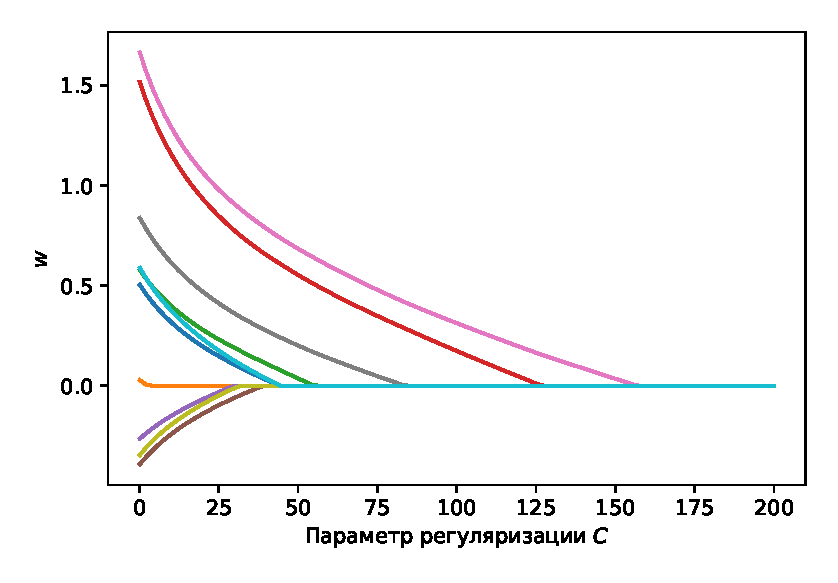
\includegraphics[width=0.5\textwidth]{../figures/log_reg_cs_exp.eps}
% 	\caption{Sample figure caption.}
% 	\label{fig:fig1}
% \end{figure}

% \subsection{Tables}
% See awesome Table~\ref{tab:table}.

% The documentation for \verb+booktabs+ (`Publication quality tables in LaTeX') is available from:
% \begin{center}
% 	\url{https://www.ctan.org/pkg/booktabs}
% \end{center}


% \begin{table}
% 	\caption{Sample table title}
% 	\centering
% 	\begin{tabular}{lll}
% 		\toprule
% 		\multicolumn{2}{c}{Part}                   \\
% 		\cmidrule(r){1-2}
% 		Name     & Description     & Size ($\mu$m) \\
% 		\midrule
% 		Dendrite & Input terminal  & $\sim$100     \\
% 		Axon     & Output terminal & $\sim$10      \\
% 		Soma     & Cell body       & up to $10^6$  \\
% 		\bottomrule
% 	\end{tabular}
% 	\label{tab:table}
% \end{table}

% \subsection{Lists}
% \begin{itemize}
% 	\item Lorem ipsum dolor sit amet
% 	\item consectetur adipiscing elit.
% 	\item Aliquam dignissim blandit est, in dictum tortor gravida eget. In ac rutrum magna.
% \end{itemize}


\bibliographystyle{unsrtnat}
\bibliography{references}

\end{document}